\section{Energy and transport as sign readouts}\label{sec:device}
\subsection{Branch-wise instantaneous energy on round quotients}
For a round slice of radius \(q\), write \(X=|Q_\Sigma|q/(4\vol)\). Use a single external Dirac species, a common local subtraction on both charge branches and half occupation at exact zero. Then the dimensionless difference \(D=q(E_{\rm vac}(+Q)-E_{\rm vac}(-Q))\), with \(Q=|Q_\Sigma|\), obeys \(D=2X\eta_0\) until the first shell and
\begin{equation}
 D=2X\eta_0-2\delta_0(X-3/2),\qquad
 \delta_0=m_+(0)-m_-(0),\quad 3/2<X<5/2 .
 \label{eq:energy}
\end{equation}
For each eigenvalue the branch energy is proportional to \(-|\lambda-sX|\). Crossing the lowest level changes the slope of the difference by \(-2\delta_0\); all higher magnitudes stay on their original side. The eta regularization gives the common initial slope \(2\eta_0\). A zero of this energy difference is therefore a property of two independently prepared instantaneous vacua. It is neither a zero eigenvalue of the spatial operator nor an occupation in a fixed initial state.

For a left order-three quotient the slope before contact is \(8/9\), and the next zero is \(X=27/14\). For an arbitrary round lens lift an isolated zero in the indicated open interval occurs exactly for one-sided cyclic actions of orders 2, 3 and 4; the three locations are \(12/7,27/14,24/11\). The order-five one-sided case has an endpoint zero at \(5/2\). Appendix~\ref{app:energy} derives this classification for any order. The finite survey through order 32 independently checks all 434 spin lifts. On a minimal round Lorentz history \(X\ge3/2\), with equality only at maximal expansion; one must state the range of radii as well as the formal interval of the energy formula.

\paragraph{A massless control.}
On a round minimal history \(q^2=c\sin(2v)\) let \(\chi=\pm1\) denote chirality and \(\xi_\alpha\) the axial coupling of species \(\alpha\). In conformal time the shell generator is \(\chi(\lambda-s\xi_\alpha b)\), \(b=3/(2\sin 2v)\). Over \(\pi/12\le v\le\pi/6\), its evolution factorizes as \(U_s=\exp[is\beta\sum_\alpha\xi_\alpha Q_{5,\alpha}/2]U_{\LC}\), where \(\beta=(3/2)\log(\tan v_f/\tan v_i)\). A single species gives identical expectations on the algebra commuting with its axial charge when the same state is prepared. With two prescribed couplings the phase can instead be relative. On the left order-three quotient the shells \(+9/2,-11/2\) have a common right spin 2. Select the left weights \(m=\pm3/2\) surviving the quotient and contract equal right weights in a particle--hole pair across these shells. Coefficients proportional to \(\sgn m\) compensate the residual reflection. Exchanging shells in the second chirality makes the two singlets have the same LC excitation energy 10, vanishing total vector and axial excitation charges, and opposite weighted axial phases. In their equal superposition the two off-diagonal Pauli measurements have means \((\cos(\Delta\xi\,\beta),s\sin(\Delta\xi\,\beta))\). At coupling difference one these are \((0.40713827,s\,0.91336654)\). The extra species and unequal couplings are inputs to this alternative device; the Nil example below uses one massive species.

\subsection{One detector used on both charges}
Take the expanding basic compact Nil background with \(a(0)=c(0)=1\), \(W=a^2c\), \(d\tau=W\,ds\) and \(u=-Q_\Sigma/(6V_0)\). Fix \(|u|=3/8,\ h=0,\ m_D=1/4,\ 0\le s\le3/2\), using the initial inverse horizontal length as energy unit. The homogeneous Einstein--scalar equations integrate exactly. Writing \(H=\sqrt{du^2+1/12}\), \(D_*=\sqrt{H^2+1/4}\), one has
\begin{equation}
 E=ac=e^{2Hs},\qquad Y=c^{-2}=\cosh(2D_*s)-(H/D_*)\sinh(2D_*s),\qquad A=a^2=E^2Y .
 \label{eq:nilhistory}
\end{equation}
Indeed \((\log c)''=-c^4/2,\ (\log a)''=c^4/2\) and both first derivatives initially equal \(H\). The metric is identical on opposite signs. The invariant density rescaling \(\Phi=\sqrt W\psi\) gives a time-independent one-particle norm. In the lowest unpaired nonzero-centre shell take one copy with \(\nu=1/(2\pi)\). Its two chiral components evolve under
\begin{equation}
 i U'_u=H_u U_u,\quad H_u=m_D W\sigma_1+(3u/2-c^2/4-\nu A)\sigma_3,\qquad U_u(0)=I.
 \label{eq:device}
\end{equation}
The LC apparatus uses \(P_i^-\), the initially negative eigenspace of \(H_u-3u\sigma_3/2\), and \(P_f^+\), the final positive eigenspace of the same charge-subtracted Hamiltonian. These two projectors are independent of the charge sign. The measured quantity is the particle-side occupation per copy
\begin{equation}
 n_u=\tr(P_f^+ U_u P_i^- U_u^\dagger).
 \label{eq:occup}
\end{equation}
No comparison of absolute dynamical phases is needed. The half-density dynamics conserves the rank-one population trace, and \(0\le n_u\le1\).

Equation~\eqref{eq:occup} gives approximately \(0.168451\) on the negative-charge branch (\(u>0\)) and \(0.042475\) on the positive-charge branch. The enclosure for the ratio \(n_{+|u|}/n_{-|u|}\) is \(3.966\pm0.000385\). Numerical integration and a separate interval-valued product of propagators distinguish numerical digits from certified error (Appendix~\ref{app:device}). Counting the corresponding hole doubles each occupation. Counting both central directions multiplies the shell result by its copy multiplicity. A single detection event is a Bernoulli result; its mean, or the distribution across identically prepared trials, distinguishes the branches statistically.

\begin{figure}[htbp]\centering
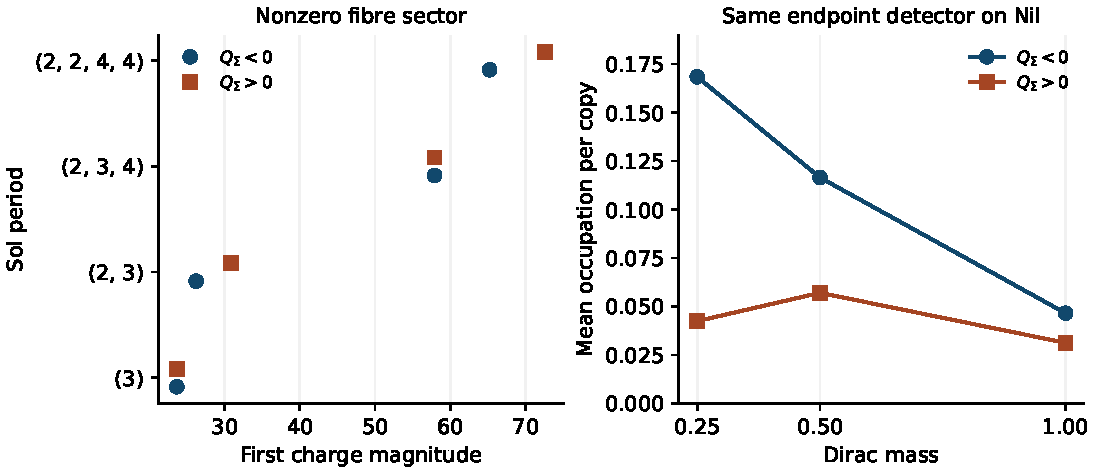
\includegraphics[width=\linewidth]{figures/readouts.pdf}
\caption{Two different comparisons. Left, the first nonzero-fibre charge magnitudes of four Sol lattices, plotted at the interval midpoints from Table~\ref{tab:sol}. Right, the particle-side mean for the same Nil shell and LC apparatus on each branch at three masses, \(h=0,\ |u|=3/8\). Lines join the calculated masses only.}
\label{fig:device}
\end{figure}

With \(m_D=0\), the massless paired two-band generator has charge dependence proportional to the identity within each Weyl block: after discarding its phase the Hamiltonian is \(\nu A\sigma_3+\sqrt{2\nu n}E\sigma_1\). A changing metric can still generate transitions, but their band probabilities are even under charge reversal. A sign-sensitive \emph{massive} finite-shell device and a massless even transition on the same space are compatible. The present calculation uses no infinite-mode Fock implementability assumption.
